%origen
\section{Origen y Antecedentes}

En 1994, se inventó el sistema de código QR por Masahiro Hara y un asociado de la empresa japonesa Denso Wave.\cite{2019_Hara}
\\
Los códigos QR fueron creados en Denso Wave Incorporated, Japón. Denso Wave es una empresa subsidiaria de Toyota. Se diseñaron con el proposito de gestionar los inventarios de piezas, en las plantas de fabricación de automóviles.  Han decidido no ejercer su derecho de patente para difundir su uso, pero la empresa posee la marca registrada del código.\cite{2014_Chang,2015_Emran_BOOK} 
\\
La empresa introdujo los códigos de barras en el método kanban de Toyota, proponiendo así un sistema de producción integrado para productos e información. ``Kanban'' se basa en la filosofía esencial de Toyota y es una herramienta para realizar el método de producción justo a tiempo. Es una hoja de especificación que se adjunta a una pieza y con ello durante todo su recorrido. Ahora bien, cuando empezó a aumentar el volumen de la producción, se tenían que procesar más hojas de especificaciones y se producían más errores humanos, ya que la entrada de datos se realizaba de manera manual a la computadora. Por esa razón, los códigos de barras se introdujeron en el ``kanban'' junto con escaners de códigos que lograba la entrada de forma automática en la computadora. Comenzó con el desarrollo del código QR en 1992. De hecho, los códigos de barras se usan ampliamente como un método de entrada, preciso, rápido y con un bajo coste en forma impresa.\cite{1998_Institute_Kore}

\begin{figure} 
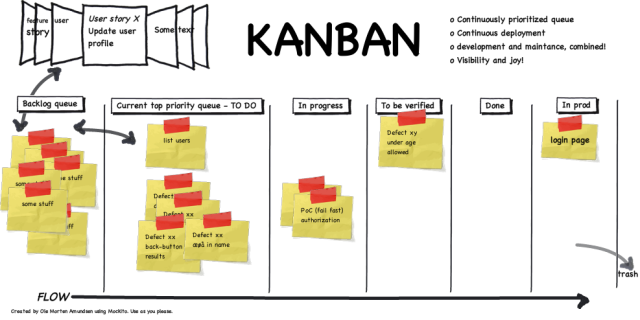
\includegraphics[width=0.6\textwidth]{kanbantoyota.png}
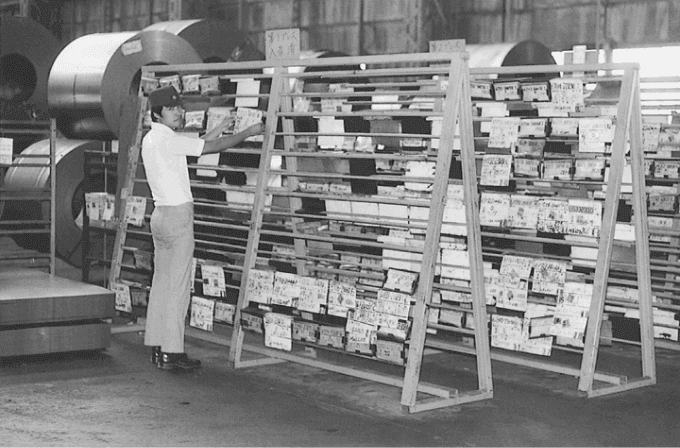
\includegraphics[width=0.4\textwidth]{kanban-board-toyota.png}
\caption{Kanban, cuyo significado es letrero o tarjeta en japonés, es un sistema de información que controla de modo armónico la fabricación de los productos necesarios en la cantidad y tiempo necesarios en cada uno de los procesos que tienen lugar tanto en el interior de la fábrica, como entre distintas empresas.}
\label{fig:kanban1}
\end{figure}

Sin embargo, las tendencias cambiaron de la producción en masa a la producción de ``bajo volumen de productos múltiples''. Para el control de producción finamente ajustado en las plantas de fabricación y, con el aumento del volumen de información manejada, se tuvieron que leer varios códigos de barras diferentes ralentizando la eficiencia de la producción y además de fatigar a los trabajadores. Se puede señalar que tras el colapso de la burbuja económica, muchas empresas buscaron calidad como diferenciación de sus productos. Por tal motivo, se deseaban mantener el control a nivel de componentes, demandando un código que pudiera imprimirse en componentes de tamaño micro como IC.\cite{2002_Hoshino}

